\documentclass[10pt,a4paper]{amsart}
% \documentclass[10pt,a4paper]{article}
\usepackage[utf8x]{inputenc}
\usepackage{ucs}
\usepackage[brazil]{babel}
\usepackage[T1]{fontenc}
\usepackage{amsmath}
\usepackage{amsfonts}
\usepackage{amssymb}
\usepackage{indentfirst}
%to bind figures in respective sections
\usepackage[section]{placeins}
%to number figures considering the section
\usepackage{chngcntr}
\counterwithin{figure}{section}

%for pseudocode
% \usepackage[]{algorithm2e}
\usepackage{algorithm}
\usepackage[noend]{algpseudocode}
\makeatletter
\def\BState{\State\hskip-\ALG@thistlm}
\makeatother
\floatname{algorithm}{Algoritmo}
\renewcommand{\algorithmicrequire}{\textbf{Entrada:}}
\renewcommand{\algorithmicensure}{\textbf{Saída:}}
\renewcommand{\algorithmicwhile}{\textbf{Enquanto}}
\renewcommand{\algorithmicdo}{\textbf{faça}}
\renewcommand{\algorithmicfor}{\textbf{Para}}
\renewcommand{\algorithmicif}{\textbf{Se}}
\renewcommand{\algorithmicthen}{\textbf{então}}

% for pretty-printed source code
\usepackage{listings}
% environment for C code
\lstnewenvironment{code}
 {\lstset{ %
     extendedchars=true,
     stringstyle=\ttfamily \scriptsize, %
     showstringspaces=false, aboveskip={1.\baselineskip}, %
     identifierstyle=\ttfamily \scriptsize \bf, %
     language=C,           %
     basicstyle=\ttfamily \small,  %\footnotesize
     numberstyle=\footnotesize, %
     % keywordstyle=\bf,       % keyword style
     tabsize=1,                 % sets default tabsize to 2 spaces
     captionpos=t,              % sets the caption-position to bottom
     breaklines=true,           % sets automatic line breaking
     breakatwhitespace=false,   % sets if automatic breaks should only happen at whitespace
     %backgroundcolor=\color{black!10},
   }
} {}

\author{Jo\~ao S. Brito Jr.\\NUSP: 5889672}
\title{Laboratório de Inteligência Artificial: \\Revisão de Crenças}
\date{\today}
\usepackage{graphicx}
\graphicspath{ {images/} }

\begin{document}

\begin{abstract}
  % Resumo
  Este documento descreve a implementação de um algoritmo de revisão de crenças. Dado um arquivo de entrada com uma base de crenças e um conjunto de sentenças para revisão, é gerada uma nova base de crenças que contém as sentenças do conjunto de revisão e a maior quantidade possível de crenças da base original mantendo a consistência.
\end{abstract}

\maketitle

% \section{Introdução}

\section{Implementação}
%   descrição da implementação
O programa implementado recebe como entrada uma base de crenças \textbf{K}, e um conjunto de sentenças para revisão \textbf{R} e cria uma base auxiliar \textbf{K'} substituindo os átomos que são comuns a \textbf{K} e \textbf{R} por novos átomos auxiliares não pertencentes a linguagem (para cada átomo $p$, substituir por $p'$).

Definimos que um conjunto de equivalências é um conjunto de cláusulas do tipo $p \equiv p'$, e utilizamos estas cláusulas para igualar um átomo a seu respectivo auxiliar.

Com a base auxiliar \textbf{K'} buscamos encontrar os maiores conjuntos de equivalência possíveis que mantenham consistente (satisfatível) a base resultante da união de \textbf{K'} e \textbf{R}.

Para cada conjunto de equivalências maximal geramos uma base revisada. Os átomos $p'$ que pertencem ao conjunto maximal são substituídos por $p$ e os que não pertencem são substituídos por $\neg ~p$.

Por fim, as possíveis bases revisadas são gravadas no arquivo de saída informado pelo usuário.

Em nossa implementação os conjuntos de equivalências maximais são obtidos através do método \emph{get\_max\_equivalence\_sets()} que recebe como entrada a lista de átomos comuns a \textbf{K} e \textbf{R}, e a base que corresponde à união de \textbf{K'} e \textbf{R}.

Este método itera por todas as combinações possíveis de elementos da lista de átomos em ordem descendente de tamanho. Para cada combinação, gera-se o conjunto de equivalências e efetua-se o teste de satisfabilidade. Se o conjunto for aprovado é adicionado a lista de conjuntos maximais.

Para evitar chamadas desnecessárias ao SAT, o procedimento ignora os conjuntos que são subconjuntos de um maximal previamente conhecido, ou que são superconjuntos de algum dos conjuntos mínimos que geram inconsistência.

A ordem descendente de tamanho das combinações foi escolhida por reduzir a quantidade de chamadas ao SAT nos testes efetuados.

\section{Instruções de execução}
O código foi implementado em \emph{Python 2.7} e utiliza a biblioteca \emph{sympy} para converter expressões lógicas para CNF e efetuar a verificação de satisfatibilidade.

Para executar, pode-se utilizar o seguinte comando:
\begin{itemize}
 \item[] \emph{python main.py <belief-base> <new-information> <revised-base>}
 \item[] ex: \emph{python main.py KB.txt R.txt result.txt}
\end{itemize}

Onde \emph{<belief-base>} é o arquivo contendo as crenças iniciais, \emph{<new-information>} contêm as sentenças para revisão e \emph{<revised-base>} é o arquivo resultado com as possíveis escolhas de bases revisadas.

\section{Testes e resultados}
%   incluir testes/ resultados e uma subseção com comentários pessoais
%   configuração dos experimentos: computador, parâmetros utilizados
% Todos os experimentos foram efetuados em uma máquina com processador Intel Core 2 Duo 2.10GHz com 4GB de memória.



% As figuras abaixo mostram os resultados obtidos:
% Fig. ~\ref{fig:mid_layer_2_10}
% \begin{figure}[ht]
%   \centering
%   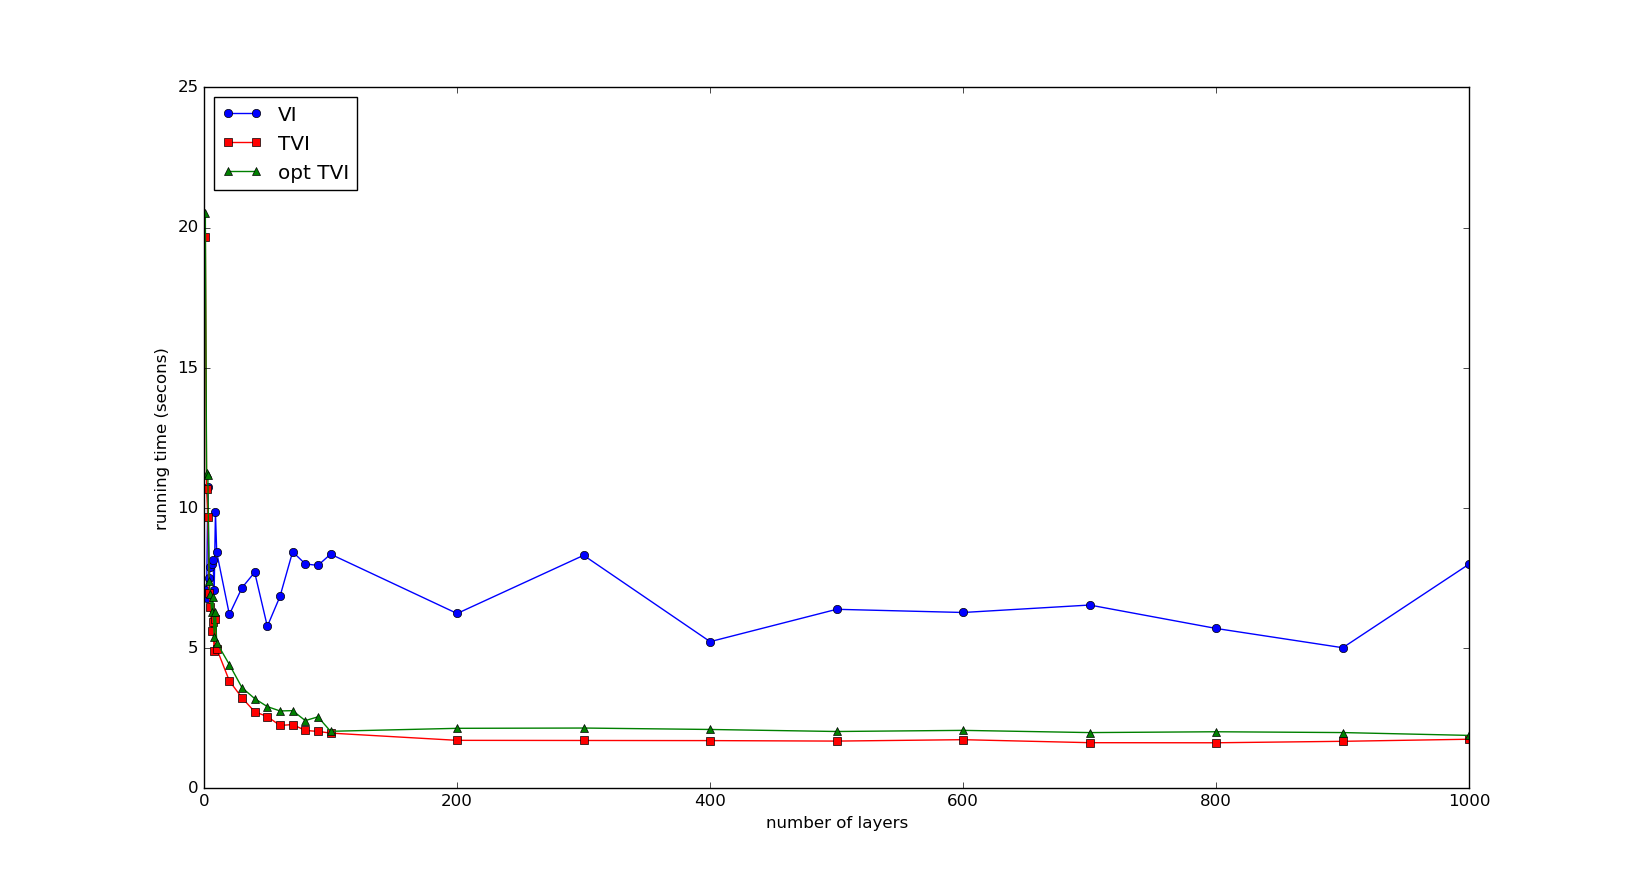
\includegraphics[width=\textwidth]{mid_layer_2_10}
%   \caption{Tempo em função do número de camadas. Problemas SSP gerados artificialmente com 5000 estados, 10 ações por estado, máximo de 10 sucessores por ação. Custo aleatório entre 2 e 10.}
%   \label{fig:mid_layer_2_10}
% \end{figure}

% \section{Conclusão}

% \begin{thebibliography}{9}
% \bibitem{dai11}
%   Dai, P., Weld, D. S., Goldsmith, J. (2011). Topological value iteration algorithms. Journal of Artificial Intelligence Research, 181-209.
% \end{thebibliography}

\end{document}
